\newpage
\section{Evaluating Overhead}
\label{sec:results}

In this section, we present the outcomes of our evaluation of \framework{}, focusing on its performance overhead in a real device while running various real world apps.  We first quantify per API call overhead of \framework{} using micro-benchmarks. And then evaluate memory and battery overhead of \framework{} was evaluated using 10 most popular apps downloaded from the Google Play Store.

All permissions requested by the apps were granted beforehand, and the apps were subjected to 10 minutes of manual usage 5 times. All experiments were conducted on a \textit{Samsung Galaxy M21} smartphone with a 2.3 GHz octa-core processor and 4 GB of RAM running Android 12. 

\mysubsubsection{API call overhead}
We measure the time elapsed during code execution by executing hooked API methods within the \texttt{Timing.measureNanoTime()} method. We observed an average overhead of 1.64 ms across different API calls. The increase in elapsed time is because of the operations performed by the hooks. For user data like contacts and camera, we experienced an overhead of 3.87 ms and 3.23 ms respectively. For tracking and clipboard user data, we observed an overhead of 0.83 ms and 1.07 ms respectively. The overhead depends on the operations performed by the respective permission-deceiving hooks. For contacts and camera APIs, we are performing intensive operations like reading a database and manipulating pixels of an image, whereas for tracking and clipboard APIs, we are simply returning a deceived string.

Many of these APIs were called several times during the app runs in our experiments. The API call overhead, however, did not impact the performance of the apps we tested in any observable manner.

\mysubsubsection{Memory Used} 
The memory utilization of the benchmarking app was measured using \textit{ADB}'s \textit{dumpsys} tool, using the \textit{Proportional Set Size (PSS)} metric. This metric captures the shared memory proportionally used by each process.

\begin{figure}[t]
    \centering
    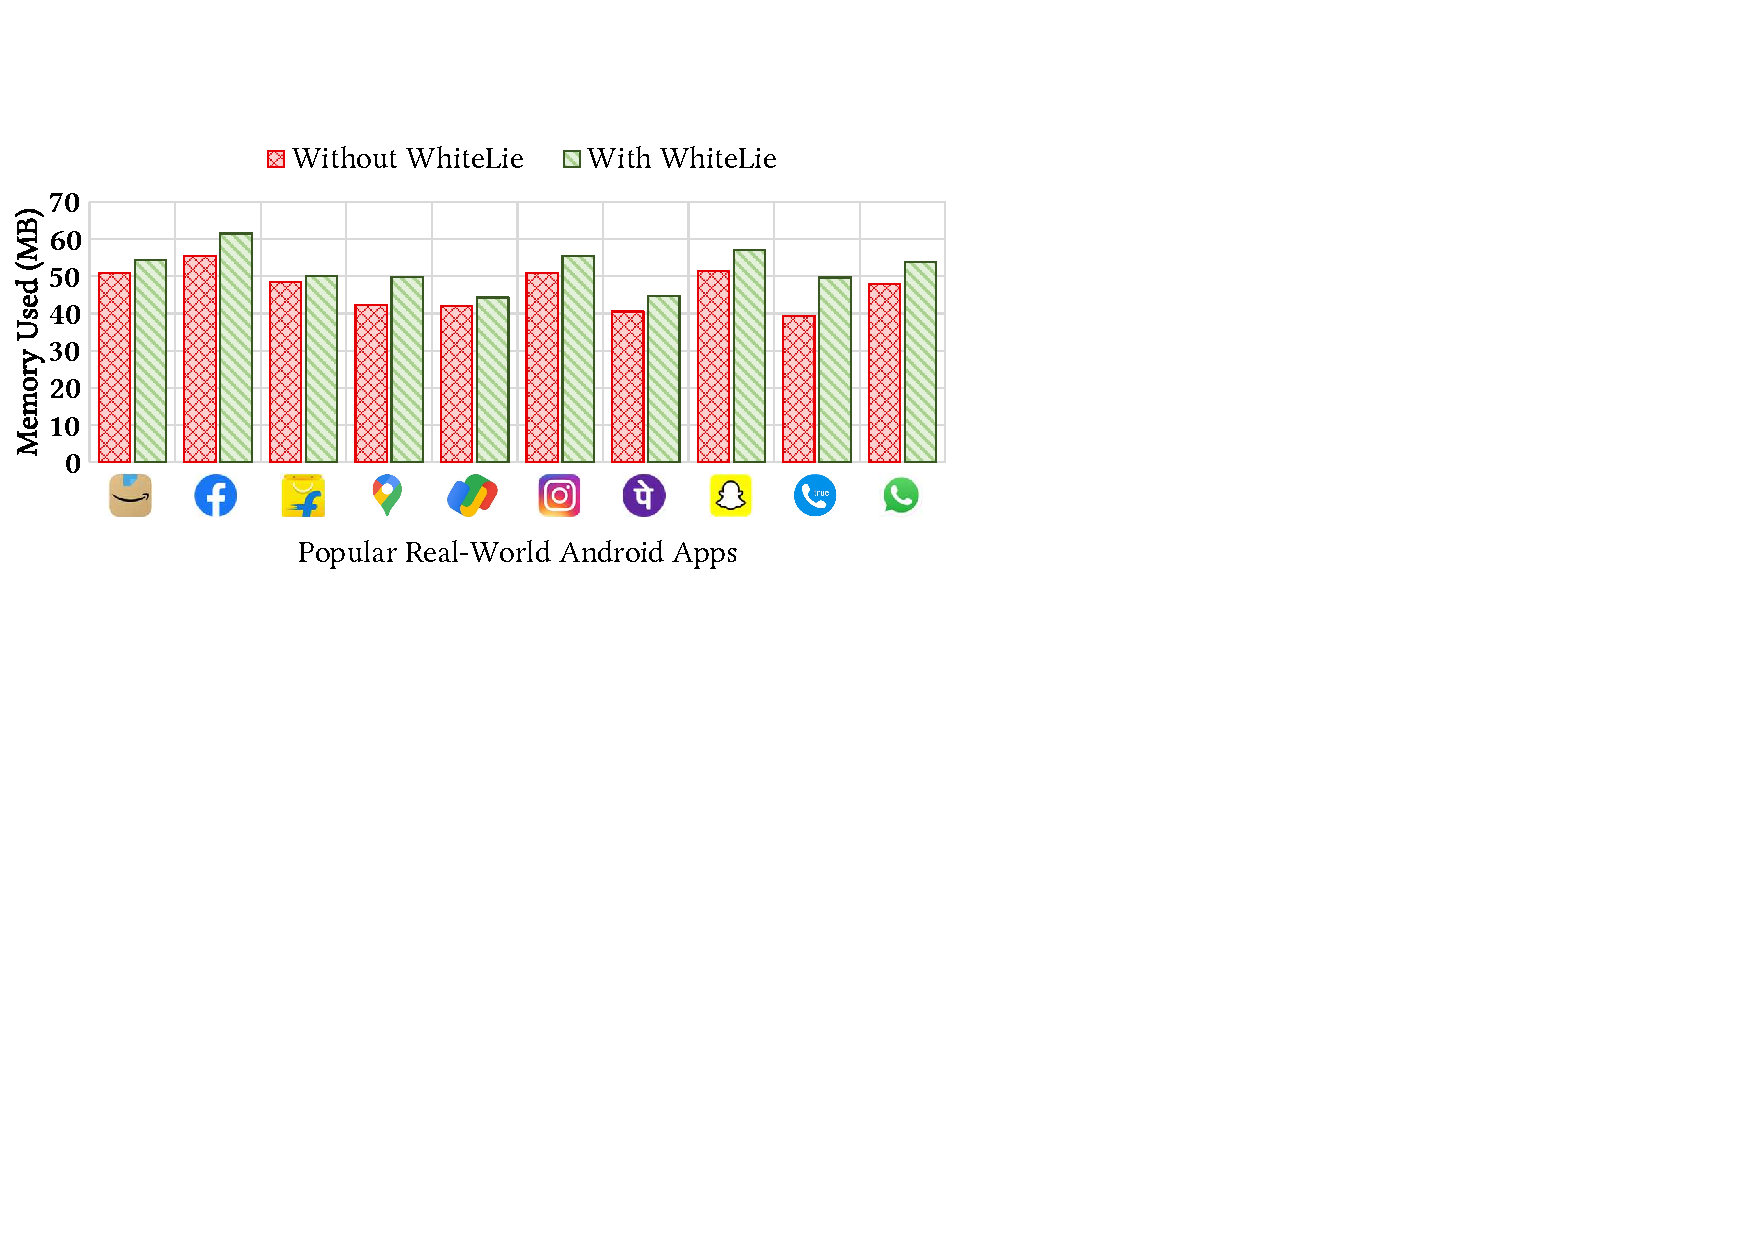
\includegraphics[width=0.8\linewidth]{Figures/Performance Evaluation/results_memory_used_target_app_real_world_apps.pdf}
    \caption{Memory used by various Android apps with and without \framework{}.}
    \label{fig:results_memUsedAll}
\end{figure}

Figure~\ref{fig:results_memUsedAll} shows that the memory overhead while using \framework{} on various real-world apps is negligible.  On average, \framework{} only incurs 5.2 MB of memory overhead. 

\mysubsubsection{Battery Discharged}
To accurately measure the device's battery usage during our experiments, we utilized the \textit{ADB}'s \textit{batterystats} tool~\cite{batterystats}. Before each experiment, we ensured a clean slate by resetting the tool. To mitigate any potential inconsistencies in battery usage statistics, we remotely connected the device via \textit{Wifi ADB}, as physically connecting it to a PC can inadvertently charge the device and yield inaccurate results.  By leveraging \texttt{batterystats}'s \textit{discharge} metric, we could quantify the amount of battery discharged since the last charge, accounting for the impact by both the target app and the system. 

\begin{figure}[t]
    \centering
    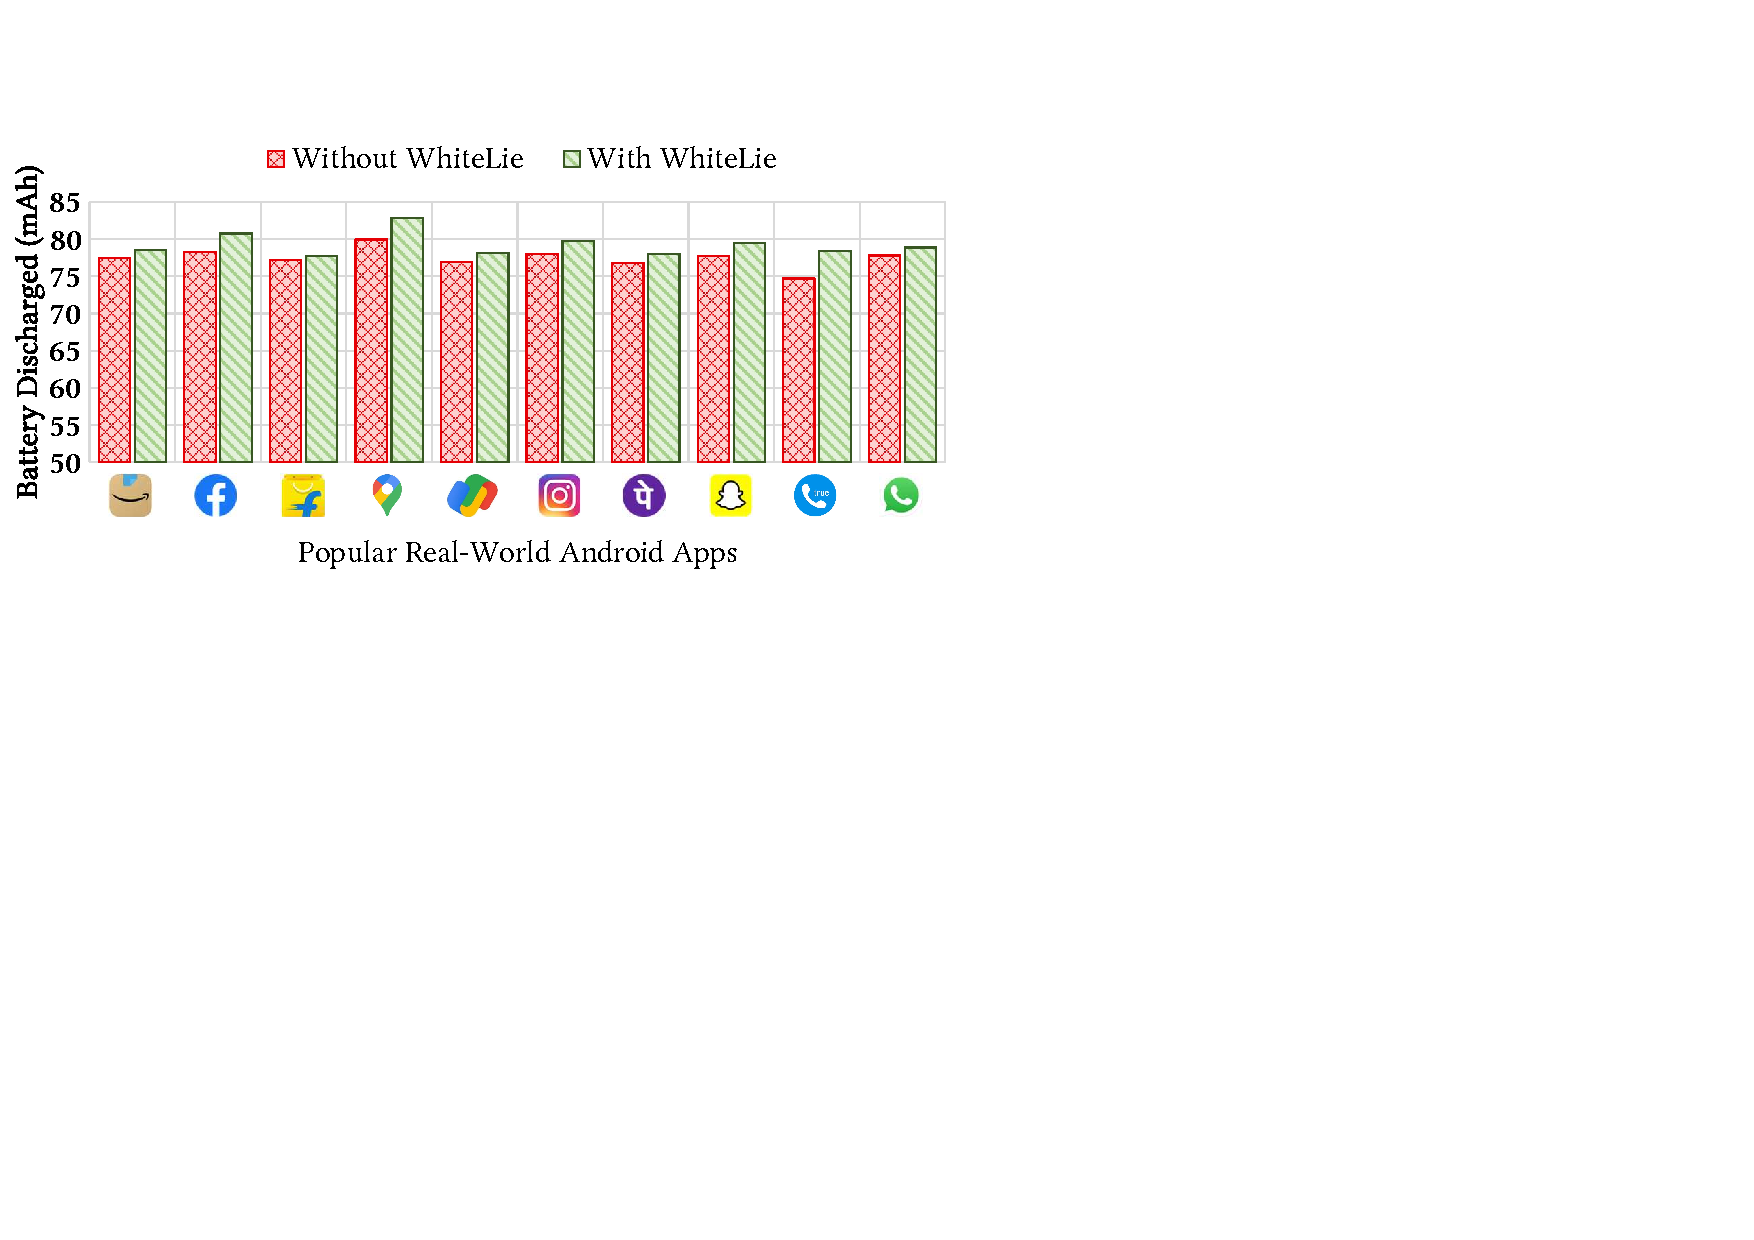
\includegraphics[width=0.8\linewidth]{Figures/Performance Evaluation/results_battery_discharged_real_world_apps.pdf}
    \caption{Battery discharged by various Android apps with and without \framework{}.}
    \label{fig:reslts_btryDschrgd}
\end{figure}

Figure \ref{fig:reslts_btryDschrgd} shows the battery drained during the  app runs with and without \framework{}. It shows that \framework{}'s impact on battery drain is negligible. An average additional discharge of approximately 1.76 mAh (2.52\%) was observed across the 5 minute runs of various apps experimented when they were run with \framework{}. 

\textit{Overall, our experiments show that \framework{}'s usage has a minimal impact on app's performance, app's memory consumption, and the device's battery drain. This shows that \framework{} is a versatile and efficient approach to protecting user privacy.}

\begin{figure}[t]
    \centering
    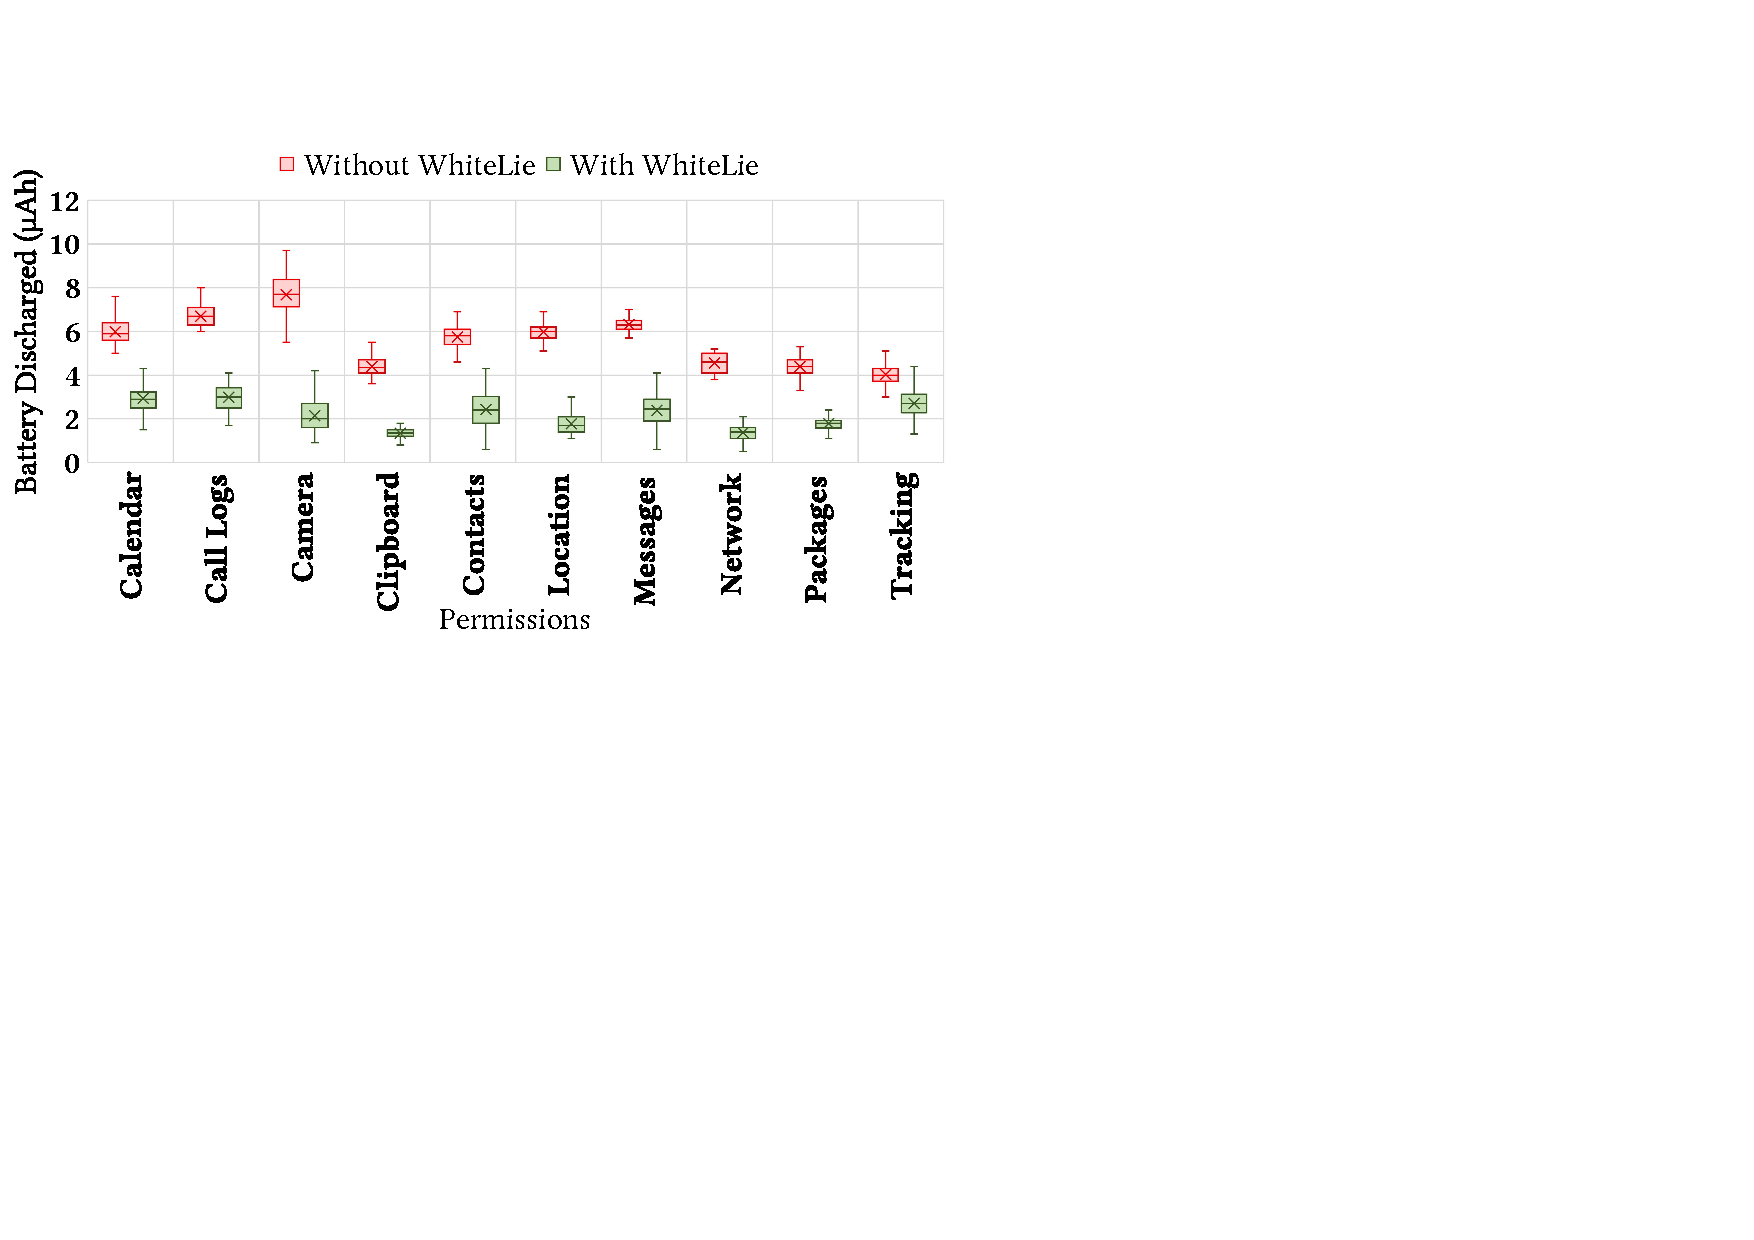
\includegraphics[width=0.8\linewidth]{Figures/Performance Evaluation/results_battery_discharged_battery_saver.pdf}
    \caption{Battery discharged by benchmarking app while fetching user data for various Permissions with and without \framework{}.}
    \label{fig:reslts_btrySaver}
\end{figure}

We further experimented with actively reducing battery drain using \framework{}. In particular, by returning \texttt{null} from the \texttt{beforeHookedMethod()}, the method calls to the original method can be blocked which can save battery consumed by sensors and other components. To examine this, we added a battery saver mode to \framework{} that selectively blocks Android API calls according to user policies.  To quantitatively measure the battery drainage, we developed a benchmarking app that performed a consecutive series of 1000 API calls to retrieve user data. We observed this approach can save an average of 4.08 $\mu{}Ah$ (60.83\%) per API call.
